\section{Resultados}

Este tópico é dedicado a apresentar os resultados, adversidades e contribuições 
alcançadas durante o desenvolvimento do estudo. Por fim, são apresentadas 
considerações sobre as limitações ocorridas no desenvolvimento deste trabalho.

\subsection{Configuração do experimento}
\label{subsection:configuracao}

\textbf{Alvo} -- Dada a matriz de referência do \citeauthor{edital_enem:2016} 
(\citeyear{edital_enem:2016}), a competência III, ``Selecionar, relacionar, 
organizar e interpretar informações, fatos, opiniões e argumentos em defesa de 
um ponto de vista.'', foi selecionada aleatoriamente, como o alvo da 
inferência indutiva dos classificadores, para teste da hipótese proposta.

\textbf{Naive Bayes} -- Para o algoritmo Naive Bayes, não foi preciso ajustar os
parâmetros, pois ele é não paramétrico.

\textbf{AdaBoost} -- O Classificador base utilizado pelo AdaBoost foi a
Árvore de decisão, com uma taxa de aprendizado configurado em 1,0 (um) e o 
número de iterações foi ajustado para 50 (cinquenta).

\textbf{Validação cruzada} -- O \textit{dataset} foi dividido em 10 conjuntos 
disjuntos com 69 textos. Os classificadores são treinados 10 vezes, cada 
vez com um conjunto diferente sendo deixado de fora para fazer a validação.

\subsection{Disposição das classes no \textit{dataset}}
\label{subsection:balanceamento}

Dada as 6 663 redações coletadas originalmente, a aplicação do método de 
limpeza e balanceamento de dados, filtrou um segundo \textit{dataset}, dispondo 
de 690 redações de temas diversificados, onde, cada classe da competência III 
possui uma amostragem de 138 redações. O Gráfico \ref{graphic:dataset_balanced} 
demonstra e destaca a disposição das classes distintas, (0.00, 0.50, 1.00, 
1.50, 2.00) sobre a competência III, bem como as disposição das classes, nas 
demais competências existentes no novo \textit{dataset}.

\begin{figure}[H]
    \begin{center}
    \begin{tikzpicture}
        \begin{axis}[
                ybar,
                width=15cm,
                height=8cm,
                bar width=11pt,
                axis lines*=left,
                ylabel=Quantidade,
                xlabel=Classes,
                symbolic x coords={0.00,0.50,1.00,1.50,2.00},
                legend style={at={(0.7,0.9)},anchor=north west},
                xtick=data,
            ]
            \addlegendentry{Compentência I}
            \addplot[draw=black, pattern color=blue, pattern=horizontal lines] coordinates{
                (0.00,91)
                (0.50,105)
                (1.00,162)
                (1.50,77)
                (2.00,255)
            };

            \addlegendentry{Compentência II}
            \addplot[draw=black, pattern color=green, pattern=vertical lines] coordinates{
                (0.00,92)
                (0.50,137)
                (1.00,249)
                (1.50,163)
                (2.00,49)
            };

            \addlegendentry{Compentência III}
            \addplot[draw=black, pattern color=red, pattern=north east lines, preaction={draw=red, line width=2pt}] coordinates{
                (0.00,138)
                (0.50,138)
                (1.00,138)
                (1.50,138)
                (2.00,138)
            };

            \addlegendentry{Compentência IV}
            \addplot[draw=black, pattern color=yellow, pattern=dots] coordinates{
                (0.00,91)
                (0.50,142)
                (1.00,307)
                (1.50,118)
                (2.00,32)
            };

            \addlegendentry{Compentência V}
            \addplot[draw=black, pattern color=gray, pattern=grid] coordinates{
                (0.00,97)
                (0.50,170)
                (1.00,149)
                (1.50,155)
                (2.00,119)
            };

        \end{axis}
    \end{tikzpicture}
    \caption{Distribuição das classes sobre a competência III de 690 redações 
    no \textit{dataset} balanceado. Cada classe da competência III possui uma 
    amostragem de 138 redações.}
    \label{graphic:dataset_balanced}
    \end{center}
\end{figure}

\subsection{Resultado da inferência indutiva}

A analise da curva ROC demonstra o poder de descriminação de cada classe, pelos 
classificadores \textit{Naive Bayes} e \textit{Adaboost}. O céu ROC ou ponto 
1,0 no vetor Y do gráfico \ref{graphic:roc}, encontram-se os pontos mais 
próximos da classificação perfeita, representa bons resultados, enquanto os 
pontos próximos de 0,5 representa um poder de classificação considerado 
aleatório. Através destes resultados, avalia-se que o poder de discriminação 
das classes de ambos os classificadores é superior ao ponto aleatório, com 
uma considerável margem de espaço, ou seja, a indução dos classificadores 
produziu informações com capacidade de distinguir as classes da competência 
III.

% Curva ROC
\begin{figure}[H]
    \begin{center}
        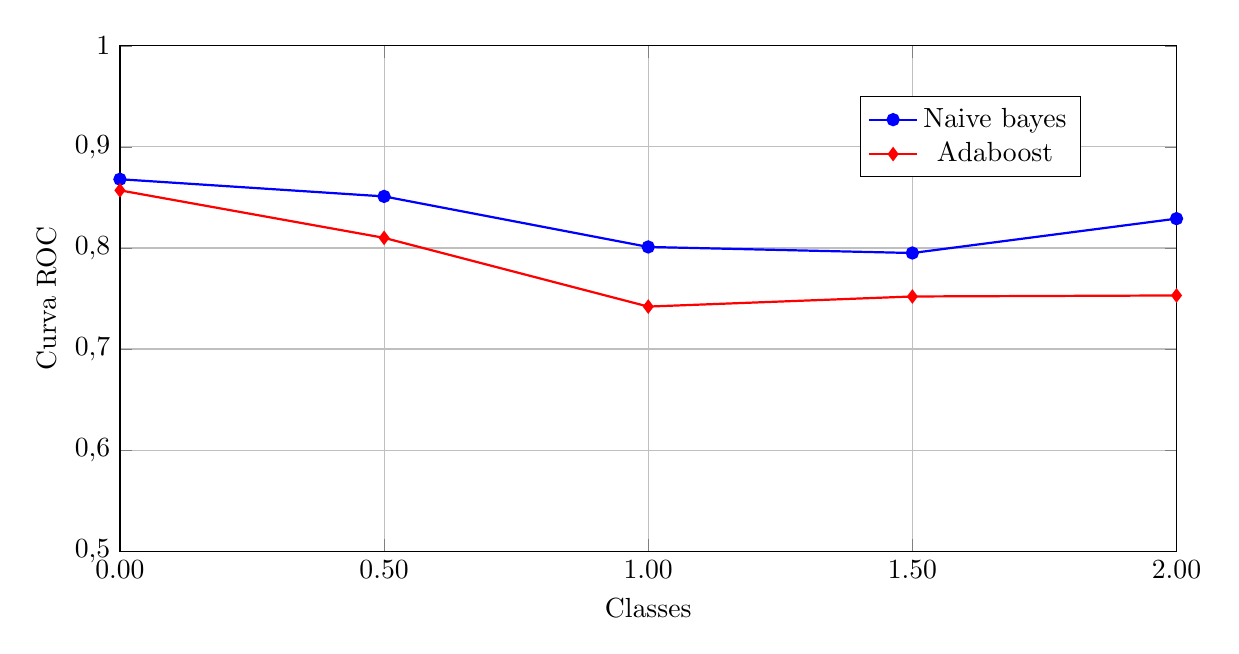
\begin{tikzpicture}
        \begin{axis}[width=15cm, 
                height=8cm, 
                grid=both, 
                ymin=0.500, ymax=1.000,
                xmin=0.00, xmax=2.00,
                ylabel={Curva ROC},
                xlabel={Classes},
                symbolic x coords={0.00, 0.50, 1.00, 1.50, 2.00},
                legend style={at={(0.7,0.9)},anchor=north west},
                xtick=data
            ]

            \addlegendentry{Naive bayes}
            \addplot[mark=*,thick,blue] coordinates {
            (0.00,0.868) 
            (0.50,0.851) 
            (1.00,0.801) 
            (1.50,0.795) 
            (2.00,0.829) 
            };

            \addlegendentry{Adaboost}
            \addplot[mark=diamond*,thick,red] coordinates {
            (0.00,0.857) 
            (0.50,0.810) 
            (1.00,0.742) 
            (1.50,0.752) 
            (2.00,0.753) 
            };

        \end{axis}
        \end{tikzpicture}
    \end{center}
    \caption{A sobreposição dos resultados da curva ROC demonstra o poder de 
    descriminação de cada classe na competência III pelos classificadores 
    \textit{Naive Bayes} e \textit{Adaboost}.}
    \label{graphic:roc}
\end{figure}

Medir adequadamente o desempenho de classificadores através da taxa de acerto, 
assume um papel importante no Aprendizado de Máquina, a \textit{acurácia} 
expressa a proporção de exemplos preditos como positivos corretamente. No 
gráfico \ref{graphic:acuracia}, está delineado os resultados da 
\textit{acurácia} de cada classe distinta, predita pelos classificadores na 
validação cruzada, com isso, dado o poder de descriminação das classes 
apresentadas no gráfico \ref{graphic:roc}, demonstra-se que os classificadores, 
\textit{Naive Bayes} e \textit{Adabost}, utilizam o conhecimento induzido 
corretamente, para rotulagem de novas amostras.

\begin{figure}[H]
    \begin{center}
        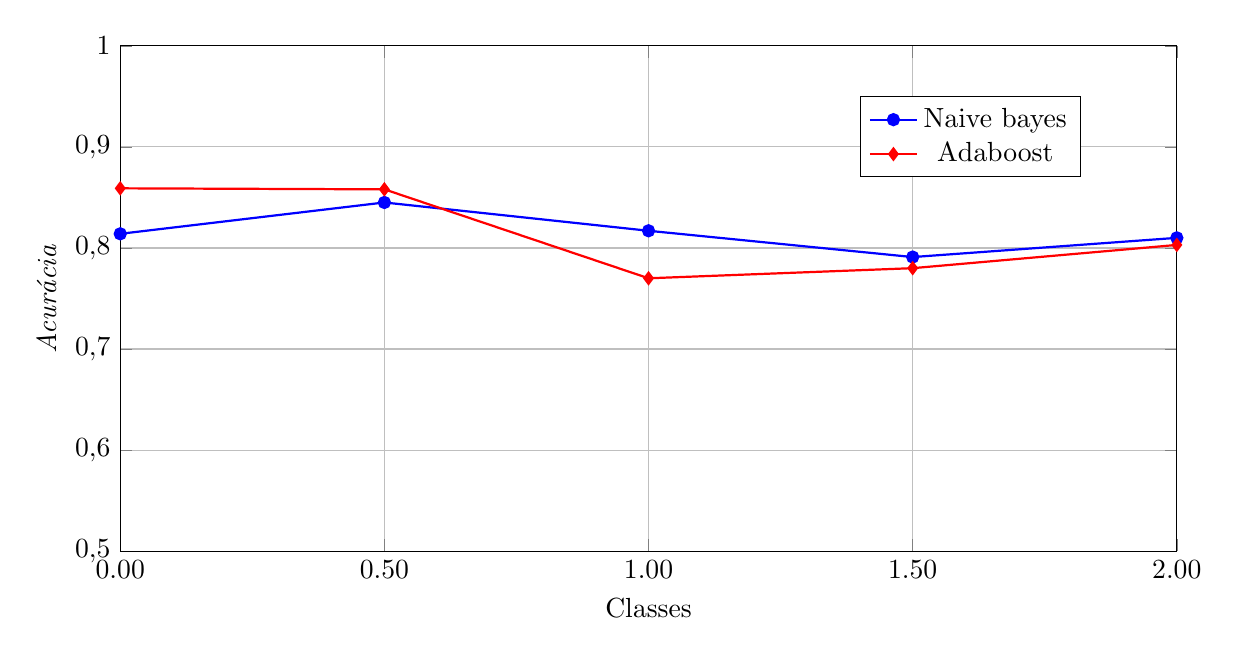
\begin{tikzpicture}
        \begin{axis}[width=15cm, 
                height=8cm, 
                grid=both, 
                ymin=0.500, ymax=1.000,
                xmin=0.00, xmax=2.00,
                ylabel={\textit{Acurácia}},
                xlabel={Classes},
                symbolic x coords={0.00, 0.50, 1.00, 1.50, 2.00}, 
                legend style={at={(0.7,0.9)},anchor=north west},
                xtick=data
            ]

            \addlegendentry{Naive bayes}
            \addplot[mark=*,thick,blue] coordinates {
            (0.00,0.814) 
            (0.50,0.845) 
            (1.00,0.817) 
            (1.50,0.791) 
            (2.00,0.810) 
            };

            \addlegendentry{Adaboost}
            \addplot[mark=diamond*,thick,red] coordinates {
            (0.00,0.859) 
            (0.50,0.858) 
            (1.00,0.770) 
            (1.50,0.780) 
            (2.00,0.803) 
            };

        \end{axis}
        \end{tikzpicture}
    \end{center}
    \caption{Os resultados da \textit{acurácia} demonstra que o poder de 
    descriminação de cada classe na competência III pelos classificadores 
    \textit{Naive Bayes} e \textit{Adaboost} está sendo utilizada corretamente 
    na rotulagem de novas amostras}
    \label{graphic:acuracia}
\end{figure}

A matriz de confusão é uma importante ferramenta, na avaliação dos resultados 
das predições, facilita visualmente o entendimento e reage aos efeitos de 
predições falsas. A análise da matriz na Tabela \ref{tab:matrix_naive_bayes} e 
\ref{tab:matrix_adaboost} respectivamente dos algoritmos \textit{Naive Bayes} e 
\textit{Adaboost} foi fundamental para a avaliação dos classificadores.

% Matriz de confusão Naive Bayes
\begin{table}[H]
    \centering
    \begin{tabular}{cc|c|c|c|c|c|c|}
    \cline{3-8}
     &  & \multicolumn{6}{c|}{\textit{Predição}} \\ \cline{3-8} 
     &  & \textbf{0.00} & \textbf{0.50} & \textbf{1.00} & \textbf{1.50} & \textbf{2.00} & $\sum_{}$  \\ \hline
    \multicolumn{1}{|c|}{} & \textbf{0.00} & \textbf{63} & 44 & 12 & 12 & 7  & \textit{138} \\ \cline{2-8} 
    \multicolumn{1}{|c|}{} & \textbf{0.50} & 3  & \textbf{99} & 33 & 1  & 2  & \textit{138} \\ \cline{2-8} 
    \multicolumn{1}{|c|}{} & \textbf{1.00} & 1  & 26 & \textbf{82} & 15 & 14 & \textit{138} \\ \cline{2-8} 
    \multicolumn{1}{|c|}{} & \textbf{1.50} & 3  & 10 & 17 & \textbf{61} & 47 & \textit{138} \\ \cline{2-8} 
    \multicolumn{1}{|c|}{} & \textbf{2.00} & 5  & 13 & 6  & 40 & \textbf{74} & \textit{138} \\ \cline{2-8} 
    \multicolumn{1}{|c|}{\multirow{-6}{*}{\textit{\rot{Atual}}}} & $\sum_{}$ & \textit{75} & \textit{192} & \textit{150} & \textit{129} & \textit{144} & \textit{\textbf{690}} \\ \hline
    \end{tabular}
    \caption{Matriz de confusão resultante da indução do classificador Naive Bayes.}
    \label{tab:matrix_naive_bayes}
\end{table}

% Matriz de confusão Adaboost
\begin{table}[H]
    \centering
    \begin{tabular}{cc|c|c|c|c|c|c|}
    \cline{3-8}
     &  & \multicolumn{6}{c|}{\textit{Predição}} \\ \cline{3-8} 
     &  & \textbf{0.00} & \textbf{0.50} & \textbf{1.00} & \textbf{1.50} & \textbf{2.00} & $\sum_{}$  \\ \hline
    \multicolumn{1}{|c|}{} & \textbf{0.00} & \textbf{99} & 18 & 10 & 9  & 2  & \textit{138} \\ \cline{2-8} 
    \multicolumn{1}{|c|}{} & \textbf{0.50} & 20 & \textbf{74} & 37 & 6  & 1  & \textit{138} \\ \cline{2-8} 
    \multicolumn{1}{|c|}{} & \textbf{1.00} & 8  & 27 & \textbf{75} & 20 & 8  & \textit{138} \\ \cline{2-8} 
    \multicolumn{1}{|c|}{} & \textbf{1.50} & 9  & 1  & 18 & \textbf{66} & 44 & \textit{138} \\ \cline{2-8} 
    \multicolumn{1}{|c|}{} & \textbf{2.00} & 7  & 5  & 13 & 50 & \textbf{63} & \textit{138} \\ \cline{2-8} 
    \multicolumn{1}{|c|}{\multirow{-6}{*}{\textit{\rot{Atual}}}} & $\sum_{}$ & \textit{143} & \textit{125} & \textit{153} & \textit{151} & \textit{118} & \textit{690} \\ \hline
    \end{tabular}
    \caption{Matriz de confusão resultante da indução do classificador Adaboost.}
    \label{tab:matrix_adaboost}
\end{table}

De acordo ainda com a análise da matriz de confusão apresentada nas Tabelas 
\ref{tab:matrix_naive_bayes} e \ref{tab:matrix_adaboost} observou--se que: 
quanto mais próximas as classes, maior é o número de confusões preditas pelos 
classificadores e quanto mais distantes as classes, menor o número de 
confusões, ou seja, ambos os classificadores tendem a confundir mais as 
classes 0,00 e 0,50, do que as classes 0,00 e 2,00, com isso, conclui-se, 
existe um padrão que pode ser visivelmente representado entre as classe 0,00 e 
2,00. Dada esta observação, o gráfico \ref{graphic:padrao} sobrepõem as tabelas 
produzidas pelo método \textit{bag-of-words} de vinte redações, onde a 
competência III foi corretamente rotulada, com as classes 0,00 e 2,00, por ambos 
os classificadores, respectivamente, uma amostragem de dez redações para cada 
classe. É perceptível que ambas possuem um comportamento similar, entretanto, a 
frequência das palavras utilizadas oscila de uma forma diferente em cada 
classe, o que demonstra o padrão existente em cada texto. 

\pgfplotsset{/pgf/number format/use comma}
\begin{figure}[H]
    \begin{center}
        \begin{tikzpicture}
        \begin{axis}[
            width=15cm, 
            height=8cm, 
            grid=both, 
            ymin=0.0, ymax=30.0,
            xmin=0, xmax=75,
            ylabel={Frequência},
            xlabel={Índice dos \textit{tokens}},
            legend style={at={(0.7,0.9)},anchor=north west}]
        
            \addplot [mark=none, color=red, dashed, legend] table[x=x, y=y, col sep=comma]{./data/0.00-0.csv};
            \addplot [mark=none, color=red, dashed] table[x=x, y=y, col sep=comma]{./data/0.00-1.csv};
            \addplot [mark=none, color=red, dashed] table[x=x, y=y, col sep=comma]{./data/0.00-2.csv};
            \addplot [mark=none, color=red, dashed] table[x=x, y=y, col sep=comma]{./data/0.00-3.csv};
            \addplot [mark=none, color=red, dashed] table[x=x, y=y, col sep=comma]{./data/0.00-4.csv};
            \addplot [mark=none, color=red, dashed] table[x=x, y=y, col sep=comma]{./data/0.00-5.csv};
            \addplot [mark=none, color=red, dashed] table[x=x, y=y, col sep=comma]{./data/0.00-6.csv};
            \addplot [mark=none, color=red, dashed] table[x=x, y=y, col sep=comma]{./data/0.00-7.csv};
            \addplot [mark=none, color=red, dashed] table[x=x, y=y, col sep=comma]{./data/0.00-8.csv};
            \addplot [mark=none, color=red, dashed] table[x=x, y=y, col sep=comma]{./data/0.00-9.csv};
            \addplot [mark=none, color=red, dashed] table[x=x, y=y, col sep=comma]{./data/0.00-10.csv};

            \addplot [mark=none, color=blue, solid, legend] table[x=x, y=y, col sep=comma]{./data/2.00-0.csv};
            \addplot [mark=none, color=blue, solid] table[x=x, y=y, col sep=comma]{./data/2.00-1.csv};
            \addplot [mark=none, color=blue, solid] table[x=x, y=y, col sep=comma]{./data/2.00-2.csv};
            \addplot [mark=none, color=blue, solid] table[x=x, y=y, col sep=comma]{./data/2.00-3.csv};
            \addplot [mark=none, color=blue, solid] table[x=x, y=y, col sep=comma]{./data/2.00-4.csv};
            \addplot [mark=none, color=blue, solid] table[x=x, y=y, col sep=comma]{./data/2.00-5.csv};
            \addplot [mark=none, color=blue, solid] table[x=x, y=y, col sep=comma]{./data/2.00-6.csv};
            \addplot [mark=none, color=blue, solid] table[x=x, y=y, col sep=comma]{./data/2.00-7.csv};
            \addplot [mark=none, color=blue, solid] table[x=x, y=y, col sep=comma]{./data/2.00-8.csv};
            \addplot [mark=none, color=blue, solid] table[x=x, y=y, col sep=comma]{./data/2.00-9.csv};
            \addplot [mark=none, color=blue, solid] table[x=x, y=y, col sep=comma]{./data/2.00-10.csv};
            \legend{Classe 0.00,,,,,,,,,,, Classe 2.00,,,,,,,,,,};
        \end{axis}
        \end{tikzpicture}
    \end{center}
    \caption{A sobreposição de vinte tabelas produzidas pelo método 
    \textit{bag-of-words} demonstra o padrão encontrado em cada texto de redação.}
    \label{graphic:padrao}
\end{figure}

Em ambos os classificadores, o resultado poderia ser melhor, caso o padrão 
encontrado nas redações, pudessem ser mensurado com maior representatividade, 
obtendo uma melhor separação entre as classes. O fato do \textit{dataset} ser 
essêncialmente composto por redações de temas diversificados, amenizou o poder 
dos classificadores na rotulagem de novas amostras, contudo, alcançou 
resultados positivos nas métricas propostas, o que corrobora com a hipótese 
proposta para este estudo.

A definição de um melhor algoritmo entre os analisados é inviável, e não 
faz parte da proposta deste trabalho. Entretanto, o classificador 
\textit{Naive Bayes} apresentou um resultado significativamente maior, no 
entanto, isto não significa que tal algoritmo seja de fato melhor que o 
\textit{Adaboost}, todavia, atestou a hipótese proposta e demonstrou que ambos 
os algoritmos, que possuem logica de predição distinta, quando induzidos, 
recuperam padrões implícitos no texto da redação. Contudo, as métricas aqui 
calculadas poderão ser utilizadas para guiar uma escolha de algoritmos para 
elaboração de trabalhos futuros.